% 2010 年湖北卷文科第 14 题：圆柱形容器内叠放三个相同小球的示意图。
% 来源 PDF：普通高考/2010/2010湖北文.pdf，SHA-256 70d7537f9072187051a41095e97fab1d72cc357ee9cd04e831da8cf99217af78。
% 原页：第 1 页（A3 三栏）第 2 栏中部，书页码 599。
% 重绘依据：照原页——容器以两条竖壁加浅灰底托表示；三个等球自上而下两两相切，
%   且都与柱壁相切（球半径等于底面半径）；柱口（顶部横线）恰在最上面一球的最高点，
%   即容器高度等于三个球的直径之和。球面用 ball 阴影表现明暗，不使用位图。
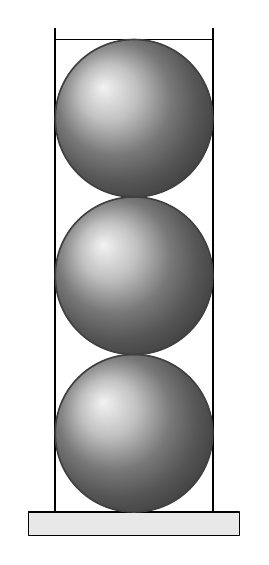
\begin{tikzpicture}[scale=1.0, semithick, line join=round]
  % 底托（浅灰扁矩形）
  \fill[gray!18] (-1.34,-0.30) rectangle (1.34,0);
  \draw (-1.34,-0.30) rectangle (1.34,0);
  % 柱壁（左右各一竖线，顶端略高出柱口，照原页）
  \draw (-1,0) -- (-1,6.14);
  \draw (1,0) -- (1,6.14);
  % 柱口：最上面一球的最高点处的横线
  \draw (-1,6) -- (1,6);
  % 三个球：半径 1，球心依次在 y=1,3,5（两两相切、与底和柱壁相切）
  \foreach \y in {1,3,5} {
    \shade[ball color=gray!65] (0,\y) circle (1);
    \draw[black!75] (0,\y) circle (1);
  }
\end{tikzpicture}
